\chapter*{Introduction}
\addcontentsline{toc}{chapter}{Introduction}

Genetic information determines the constitution and function of the cells. However, genetically identical cells show differences, such as cells from our skin and our neurons. This is explained by the mechanisms of gene regulation that determine the levels of expression of the different genes, that may change e.g. according to environmental signals even for identical cells. The chemical reactions that regulate gene expression are, at a fundamental level, collisions between diffusing molecules that occur randomly. Furthermore, some of the molecules involved (such as mRNA molecules), are present at low numbers increasing the randomness.

It is surprising how all these random chemical reactions are able to determine such complex and synchronized patterns in living beings. There must be sophisticated mechanisms in the genetic circuits that allow them to work properly regardless of the presence of noise. It is even more surprising that living beings have taken advantage of noise to in certain mechanisms that are favored by having variability.

It has been observed that even clonal populations under the same environmental conditions have very different levels of expressions \cite{elowitz02} \cite{pedraza05}. Fig. \ref{fig:int-noise1} show the varying levels of expression of genes, measured by flourescence, of genetically identical cells under the same conditions. The expression of certain gene is proportional to the intensity of a color. Thus, the variability in the colors among cells show that the fluorescent proteins are expressed at different levels. These evidences have shown that noise is inherent to biological systems and thus it is important to study it.

\begin{figure}[H]
  \centering
  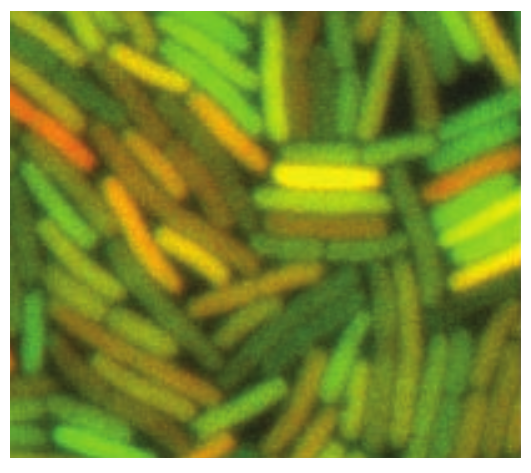
\includegraphics[width=8cm]{int-noise1}
  \caption[Examples of noise in gene expression]{\label{fig:int-noise1} . Examples of noise in gene expression for clonal population under identical environmental conditions. (left) An image taken by fluoresence microscopy of a population of bacteria. The large variation in the colors between the cells shows how large is the noise. (right) Scatter of the levels of expression, measured as fluorescence counts of two different genes. Each point represent an individual cell. The red lines show the average. The levels of expression show huge variations relative to the average. From \cite{elowitz02} (left) and \cite{pedraza05} (right).}
\end{figure}

In addition to the noticeable effect of noise. Some works have considered genetic circuits where noise plays an important role. In \cite{arkin98}, a genetic circuit that determines the mechanism by which the lambda phage virus will infect bacteria is studied. Fig. \ref{fig:int-lambda} summarizes the mechanism. When the phage infects the bacteria and introduces its genetic material there are two possibilities. In the lytic phase, the virus uses the cell to replicate its DNA and produce many viruses and then kill the bacteria. In the lysogenic phase the viral DNA is inserted in the bacterial chromosome and replicated together with the bacterial DNA. Under certain conditions, it can turn to the lytic phase and produce viruses that kill the bacteria.

It turns out that the virus decides randomly which phase to follow, with probabilities that are weighted by conditions such as the ratio between viruses and bacteria and stress signals. This is more efficient because if all viruses would take the lytic path, all the bacteria would die and they would not be able to replicate anymore. It would not also be advantageous for all the viral DNA to be hidden in the chromosomes of the bacteria. Therefore, evolution has designed this circuit to exploit noise.

\begin{figure}[H]
  \centering
  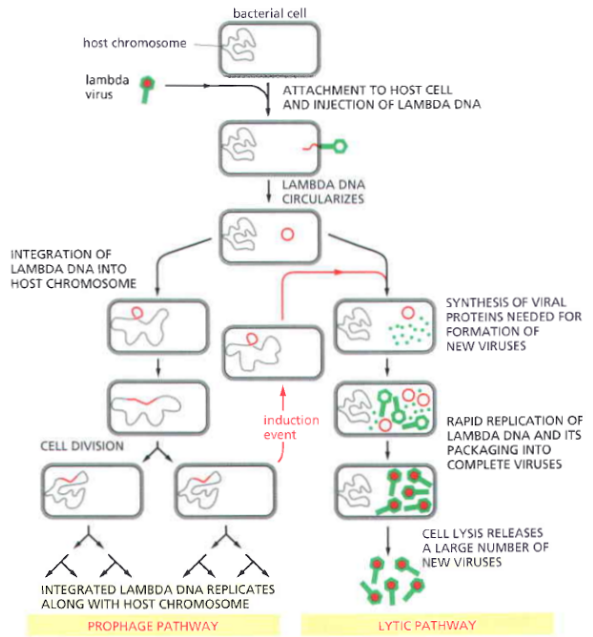
\includegraphics[width=8cm]{int-lambda}
  \caption[Life cycle of lambda phage]{\label{fig:int-lambda} The life cycle of lambda phage. When its DNA is injected into the cell it takes either the lytic or the prophage (or lysogenic) pathway. If the virus is in the lysogenic phase, it can switch back to the lytic phase. Taken from \cite{alberts08}.}
\end{figure}

Other function in which noise plays an important role is on the adaptation to changing environments. For each environmental condition there is an optimal phenotype. If the environment was fixed, the best strategy for a population would be to pick the optimal phenotype. However, the outer conditions may vary randomly and with an uncertain frequence. If the strategy for the cells were to synchronize their phenotypes with the changing environments, they would need to sense it regularly and this will have a high energetic cost. The less costly strategy is choosing the phenotype randomly, without performing any measurement. ???? have proven that what happens is a combination of both strategies. Cells choose randomly between phenotypes with a higher bias for phenotype that matches with more efficiency the measured environment. Besides, the precision when sensing the environment is chosen according the relation with the energetic cost. This is advantageous because it lowers the energetic cost of precise sensing and also allows the population to be prepared for sudden changes in the environment.

\todo[inline]{Articles of changing environments, include some figures}

On the other hand, there are biological functions that have to be very synchronized regardless of noise. For example, cell differentiation in developing embryos is determined by the levels of expression of certain genes that are subjected to noise. The circuits regulating this function must be robust to noise, meaning that they must be able to work properly regardless of its presence. This happens in many regulatory pathways. Some of the strategies that ensure that important proteins are expressed exactly when needed and at the needed levels include redundancy in genes, checkpoints in the cascade events and cooperation in the expression between individuals of a population (i.e. not every cell in the population needs to be active at the same rate) \cite{mcadams99}

\todo[inline]{Read and explain more about this}

The inherent fluctuations in each genetic component ocurring as a consequence of the discrete nature of the components has been called intrinsic noise \cite{elowitz02}. However, cells respond to environmental signals that may also vary randomly, or their growth may be irregular. Such factors introduce random fluctuations that affect all components of the cell in a correlated way. These have been called global, or extrinsic noise \cite{elowitz02} \cite{pedraza05}. 

Stochasticity, or noise, in biological circuits occurs due to of fluctuations during transcription, translation \cite{kaern05} and other processes that affect gene expression. As a consequence of noise, genetically identical cells and on the same environment may have notorious phenotypical variations \cite{kaern05} \cite{elowitz02} \cite{pedraza05}. This noise has been classified in two groups: intrinsic and extrinsic \cite{elowitz02} \cite{paulsson05}. The former is the variability inherent to systems with discrete components and low numbers (e.g. RNA and proteins). The latter is related to external factors as environmental fluctuations, cell growing and cell division.

Recent works have shown the importance of noise for living beings. They have adapted their genetic circuits to develop their respective functions correctly regardless of its presence (robustness) \cite{alon99}, or to take advantage of it to produce variability \cite{arkin98}. Also, when designing synthetic genetic circuits it is important to consider the stochasticity that the circuit may have.

For those reasons, in the last years, several stochastic models of gene expression have been developed. In a pioneer work, Thattai and van Oudenaarden \cite{thattai01} a linearized model for intrinsic noise in the amounts of RNA and proteins that can be applied to some basic motifs. Also, Pedraza and van Oudenaarden \cite{pedraza05} developed a model that includes extrinsic noise and showed how fluctuations are propagated through a cascade of regulation.

Most recent models have focused in other aspects that could induce noise. For instance, the bursting in the production of the molecules involved in gene expression, their senescence \cite{pedraza08}, and the partition of molecules during cell division \cite{huh11a} \cite{huh11b}. One of the most important conclusions of these works is that when considering different factors, the behavior of noise is similar. Therefore, by studying only the fluctuations it is difficult to know the mechanisms that produce them.

Altought many important results have been made, most of the models used are linearized around the fixed points due to the non-linearity of the equations used to model molecular kinetics. With this, information about the full dynamics of fluctuations. it would be useful then to develop stochastic models that consider the non-linearities, that include the time evolution of noise and that consider more factors like the cell growing and division together with gene expression.
